% ========================================
% IEEE Internship Report - Pneumonia Detection
% ========================================
\documentclass[conference]{IEEEtran}
\IEEEoverridecommandlockouts

% ========================================
% PACKAGES
% ========================================
\usepackage{cite}
\usepackage{amsmath,amssymb,amsfonts}
\usepackage{algorithmic}
\usepackage{graphicx}
\usepackage{textcomp}
\usepackage{xcolor}
\usepackage{url}
\usepackage{booktabs} % Required for toprule, midrule, bottomrule
\usepackage{multirow}
\usepackage{array}
\usepackage{float}    % Required for [H] table placement
\usepackage{svg}
\usepackage{tikz}
\usetikzlibrary{shapes,arrows,positioning}
\usepackage{verbatim}

% ========================================
% BIBLIOGRAPHY SETUP
% ========================================
\def\BibTeX{{\rm B\kern-.05em{\sc i\kern-.025em b}\kern-.08em
    T\kern-.1667em\lower.7ex\hbox{E}\kern-.125emX}}

% ========================================
% DOCUMENT BEGIN
% ========================================
\begin{document}

% ========================================
% TITLE AND AUTHOR
% ========================================
\title{Pneumonia Detection from Chest X-Ray Images Using Deep Learning: A Custom CNN Architecture}

\author{\IEEEauthorblockN{Lotti Hareesh}
\IEEEauthorblockA{\textit{Summer Intern} \\
\textit{Department of Computer Science} \\
RGUKT Nuzvid \\
Nuzvid, India \\
ID: N200359 \\
n200359@rguktn.ac.in}}

\maketitle

% ========================================
% ABSTRACT
% ========================================
\begin{abstract}
This paper presents an extensive study on the use of deep learning for the automated detection of pneumonia from chest X-ray images. The study utilizes a custom Convolutional Neural Network (CNN) architecture to classify images as 'Normal' or 'Pneumonia'. The dataset contains 5,863 X-ray images and exhibits a notable class imbalance. The final model achieves a test accuracy of 90.4\% with a precision of 93\% for pneumonia detection and 87\% for normal cases. The work demonstrates the effectiveness of custom CNN architectures in medical image classification and addresses the challenge of imbalanced datasets through data augmentation. The implementation uses the TensorFlow/Keras framework with advanced regularization techniques like Batch Normalization and an adaptive learning rate strategy to enhance model generalization.
\end{abstract}

% ========================================
% KEYWORDS
% ========================================
\begin{IEEEkeywords}
Deep Learning, Medical Image Analysis, Pneumonia Detection, Convolutional Neural Networks, Custom CNN Architecture, TensorFlow, Keras, Data Augmentation
\end{IEEEkeywords}

% ========================================
% 1. INTRODUCTION
% ========================================
\section{Introduction}

Pneumonia remains one of the leading causes of mortality worldwide, particularly affecting children and elderly populations. Early and accurate diagnosis is crucial for effective treatment and improved patient outcomes. Traditional diagnosis relies heavily on radiologists' interpretation of chest X-ray images, which can be time-consuming and subject to human error. With the development of deep learning methods, new opportunities are being brought for automated analysis of medical images that provide the potential for accelerated, more uniform, and possibly even more accurate diagnoses.

This internship project aims at creating an automatic pneumonia detection system based on chest X-ray images using deep learning methods. The core goal is to design a robust classifier that can distinguish between normal chest X-rays and those showing pneumonia. The study utilizes a custom CNN architecture specifically designed for medical image classification, incorporating advanced regularization techniques and comprehensive data augmentation to handle the challenges of medical imaging datasets.

% =======================================
% 2. LITERATURE SURVEY
% ========================================
\section{Literature Survey}

State-of-the-art progress in deep learning has shown spectacular success in medical image analysis. Transfer learning has proven to be a very effective strategy for medical imaging tasks, where big annotated datasets are not available. It has been proven that pre-trained models such as VGG16, ResNet, and DenseNet can be successfully used for medical image classification tasks.

The intersection of medical care and artificial intelligence has created new opportunities for computerized medical diagnosis. Deep learning techniques in medicine have demonstrated encouraging performance in a wide range of medical imaging applications, with chest X-ray analysis being one of the hottest research topics.

Some researchers have investigated pneumonia detection on chest X-ray images. Kermany et al. established a large chest X-ray dataset and proved that deep learning models can be used for medical diagnosis. Wang et al. constructed a large chest X-ray database and set benchmarks for weakly-supervised classification and localization of common thorax diseases. Rajpurkar et al. introduced CheXNet, a 121-layer DenseNet model, which reached radiologist-level performance on detecting pneumonia.

Application of data augmentation methods in medical images has proven to enhance model performance and generalizability. Methods like random rotation, flipping horizontally, and color jittering are used to overcome the scarcity of medical imaging data while preserving the integrity of diagnostic information. Best practices for deep learning in medical imaging have been derived, supplying deep learning guidance for developing resilient and trustworthy medical AI systems.

The MIMIC-CXR database has also made an important contribution to chest X-ray analysis research in the form of a large, publicly accessible database of labeled chest radiographs for training and testing deep learning models. 

% ========================================
% 3. METHODOLOGY
% ========================================
\section{Methodology}

\subsection{Model Architecture}
The research employs a custom 5-layer Convolutional Neural Network specifically designed for medical image classification. The architecture consists of progressive convolutional layers with increasing filter sizes, followed by fully connected layers for binary classification. The complete architecture is illustrated in Figure \ref{fig:model_architecture}.

Key architectural components:
\begin{itemize}
    \item \textbf{Input Layer}: 150×150×1 grayscale images for consistent processing
    \item \textbf{Convolutional Layers}: 5 Conv2D layers with filter sizes 32, 64, 64, 128, and 256
    \item \textbf{Batch Normalization}: Applied after each convolutional layer for stable training
    \item \textbf{MaxPooling}: 2×2 pooling layers for dimensionality reduction
    \item \textbf{Dropout}: Strategic dropout layers (0.1, 0.2) to prevent overfitting
    \item \textbf{Flatten Layer}: Converts 2D feature maps to 1D vector
    \item \textbf{Dense Layers}: 128-unit hidden layer with dropout (0.2)
    \item \textbf{Output Layer}: Single sigmoid unit for binary classification
\end{itemize}

The architecture follows a progressive design pattern where each convolutional block increases in complexity:
\begin{enumerate}
    \item \textbf{Block 1}: 32 filters with 3×3 kernels, batch normalization, and max pooling
    \item \textbf{Block 2}: 64 filters with dropout (0.1) for regularization
    \item \textbf{Block 3}: 64 filters maintaining feature complexity
    \item \textbf{Block 4}: 128 filters with increased dropout (0.2)
    \item \textbf{Block 5}: 256 filters for high-level feature extraction
\end{enumerate}

% CNN Architecture Diagram
\begin{figure}[!ht]
\centering
\resizebox{\columnwidth}{!}{%
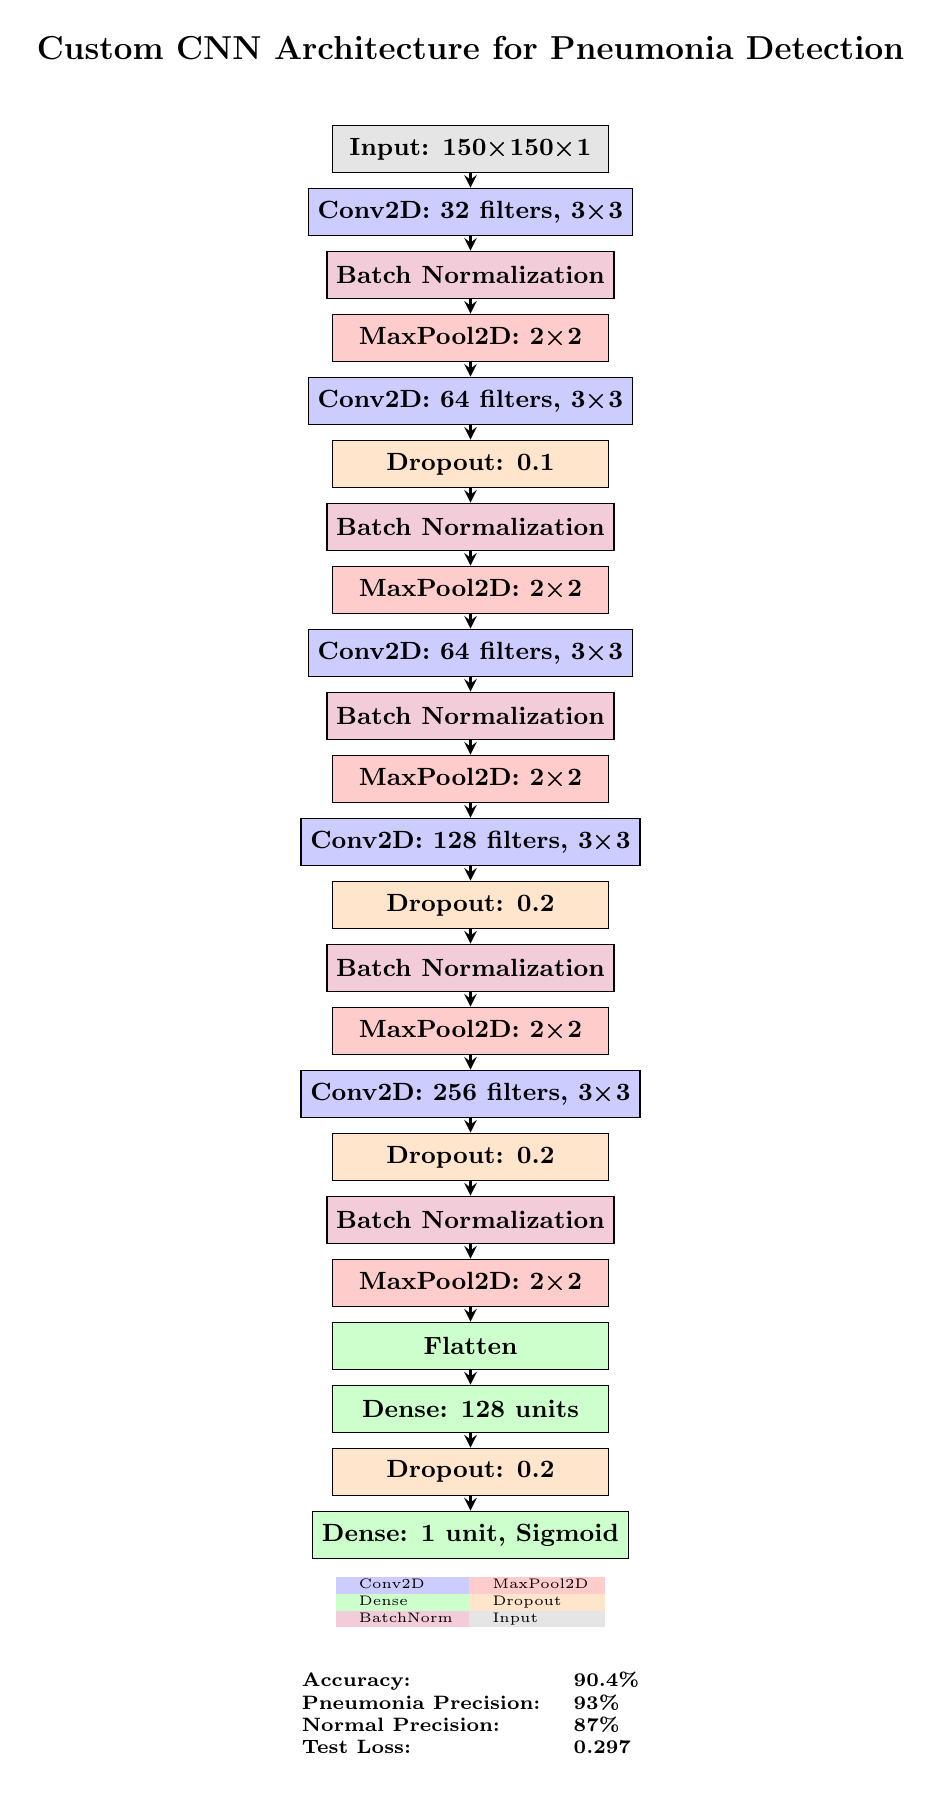
\begin{tikzpicture}[
    node distance=0.3cm,
    auto,
    thick,
    conv/.style={rectangle,fill=blue!20,draw=black,line width=0.5pt,minimum width=3.5cm,minimum height=0.6cm,font=\small\bfseries,align=center},
    pool/.style={rectangle,fill=red!20,draw=black,line width=0.5pt,minimum width=3.5cm,minimum height=0.6cm,font=\small\bfseries,align=center},
    dense/.style={rectangle,fill=green!20,draw=black,line width=0.5pt,minimum width=3.5cm,minimum height=0.6cm,font=\small\bfseries,align=center},
    dropout/.style={rectangle,fill=orange!20,draw=black,line width=0.5pt,minimum width=3.5cm,minimum height=0.6cm,font=\small\bfseries,align=center},
    batch/.style={rectangle,fill=purple!20,draw=black,line width=0.5pt,minimum width=3.5cm,minimum height=0.6cm,font=\small\bfseries,align=center},
    input/.style={rectangle,fill=gray!20,draw=black,line width=0.5pt,minimum width=3.5cm,minimum height=0.6cm,font=\small\bfseries,align=center},
    arrow/.style={->,>=stealth,thick,black,line width=1pt}
]

% Title
\node[above=0.2cm,font=\large\bfseries,align=center] at (0,0) {Custom CNN Architecture for Pneumonia Detection};

% Input Layer
\node[input] (input) at (0,-0.8) {Input: 150×150×1};

% Conv Block 1
\node[conv] (conv1) at (0,-1.6) {Conv2D: 32 filters, 3×3};
\node[batch] (bn1) at (0,-2.4) {Batch Normalization};
\node[pool] (pool1) at (0,-3.2) {MaxPool2D: 2×2};

% Conv Block 2
\node[conv] (conv2) at (0,-4.0) {Conv2D: 64 filters, 3×3};
\node[dropout] (drop1) at (0,-4.8) {Dropout: 0.1};
\node[batch] (bn2) at (0,-5.6) {Batch Normalization};
\node[pool] (pool2) at (0,-6.4) {MaxPool2D: 2×2};

% Conv Block 3
\node[conv] (conv3) at (0,-7.2) {Conv2D: 64 filters, 3×3};
\node[batch] (bn3) at (0,-8.0) {Batch Normalization};
\node[pool] (pool3) at (0,-8.8) {MaxPool2D: 2×2};

% Conv Block 4
\node[conv] (conv4) at (0,-9.6) {Conv2D: 128 filters, 3×3};
\node[dropout] (drop2) at (0,-10.4) {Dropout: 0.2};
\node[batch] (bn4) at (0,-11.2) {Batch Normalization};
\node[pool] (pool4) at (0,-12.0) {MaxPool2D: 2×2};

% Conv Block 5
\node[conv] (conv5) at (0,-12.8) {Conv2D: 256 filters, 3×3};
\node[dropout] (drop3) at (0,-13.6) {Dropout: 0.2};
\node[batch] (bn5) at (0,-14.4) {Batch Normalization};
\node[pool] (pool5) at (0,-15.2) {MaxPool2D: 2×2};

% Flatten
\node[dense] (flatten) at (0,-16.0) {Flatten};

% Dense Layers
\node[dense] (dense1) at (0,-16.8) {Dense: 128 units};
\node[dropout] (drop4) at (0,-17.6) {Dropout: 0.2};
\node[dense] (output) at (0,-18.4) {Dense: 1 unit, Sigmoid};

% Vertical Arrows
\draw[arrow] (input) -- (conv1);
\draw[arrow] (conv1) -- (bn1);
\draw[arrow] (bn1) -- (pool1);
\draw[arrow] (pool1) -- (conv2);
\draw[arrow] (conv2) -- (drop1);
\draw[arrow] (drop1) -- (bn2);
\draw[arrow] (bn2) -- (pool2);
\draw[arrow] (pool2) -- (conv3);
\draw[arrow] (conv3) -- (bn3);
\draw[arrow] (bn3) -- (pool3);
\draw[arrow] (pool3) -- (conv4);
\draw[arrow] (conv4) -- (drop2);
\draw[arrow] (drop2) -- (bn4);
\draw[arrow] (bn4) -- (pool4);
\draw[arrow] (pool4) -- (conv5);
\draw[arrow] (conv5) -- (drop3);
\draw[arrow] (drop3) -- (bn5);
\draw[arrow] (bn5) -- (pool5);
\draw[arrow] (pool5) -- (flatten);
\draw[arrow] (flatten) -- (dense1);
\draw[arrow] (dense1) -- (drop4);
\draw[arrow] (drop4) -- (output);

% Legend
\node[below=0.1cm of output,anchor=north,font=\tiny] (legend) {
\begin{tabular}{ll}
\cellcolor{blue!20} Conv2D & \cellcolor{red!20} MaxPool2D \\
\cellcolor{green!20} Dense & \cellcolor{orange!20} Dropout \\
\cellcolor{purple!20} BatchNorm & \cellcolor{gray!20} Input \\
\end{tabular}
};

% Performance metrics
\node[below=0.3cm of legend,anchor=north,font=\scriptsize\bfseries] (metrics) {
\begin{tabular}{ll}
Accuracy: & 90.4\% \\
Pneumonia Precision: & 93\% \\
Normal Precision: & 87\% \\
Test Loss: & 0.297 \\
\end{tabular}
};

\end{tikzpicture}%
}
\caption{Custom CNN architecture for pneumonia classification. The model consists of 5 convolutional layers with progressive filter sizes, batch normalization, and dropout regularization for robust medical image classification. The architecture demonstrates a systematic approach to feature extraction and classification.}
\label{fig:model_architecture}
\end{figure}

\subsection{Training Strategy}
The training process uses various optimization strategies:
\begin{itemize}
    \item \textbf{Loss Function}: Binary cross-entropy loss for binary classification
    \item \textbf{Optimizer}: RMSprop optimizer with adaptive learning rate reduction
    \item \textbf{Learning Rate Reduction}: ReduceLROnPlateau callback for dynamic learning rate adjustment
    \item \textbf{Data Augmentation}: Comprehensive augmentation including rotation, zoom, and flipping
    \item \textbf{Reproducibility}: Fixed random seeds for consistent results
\end{itemize}

% ========================================
% 4. DATASETS
% ========================================
\section{Datasets}

\subsection{Dataset Description}
The experiment employs a chest X-ray dataset of 5,863 images, which are split into training, validation, and test sets. The dataset is organized into 3 folders (train, test, val) with subfolders for each image category (Pneumonia/Normal). The data exhibits class imbalance with more pneumonia cases than normal cases. All images are resized to 150×150 pixels for consistent processing.

% [FIGURE 1: Dataset Distribution Chart]
\begin{figure}[H]
\centering
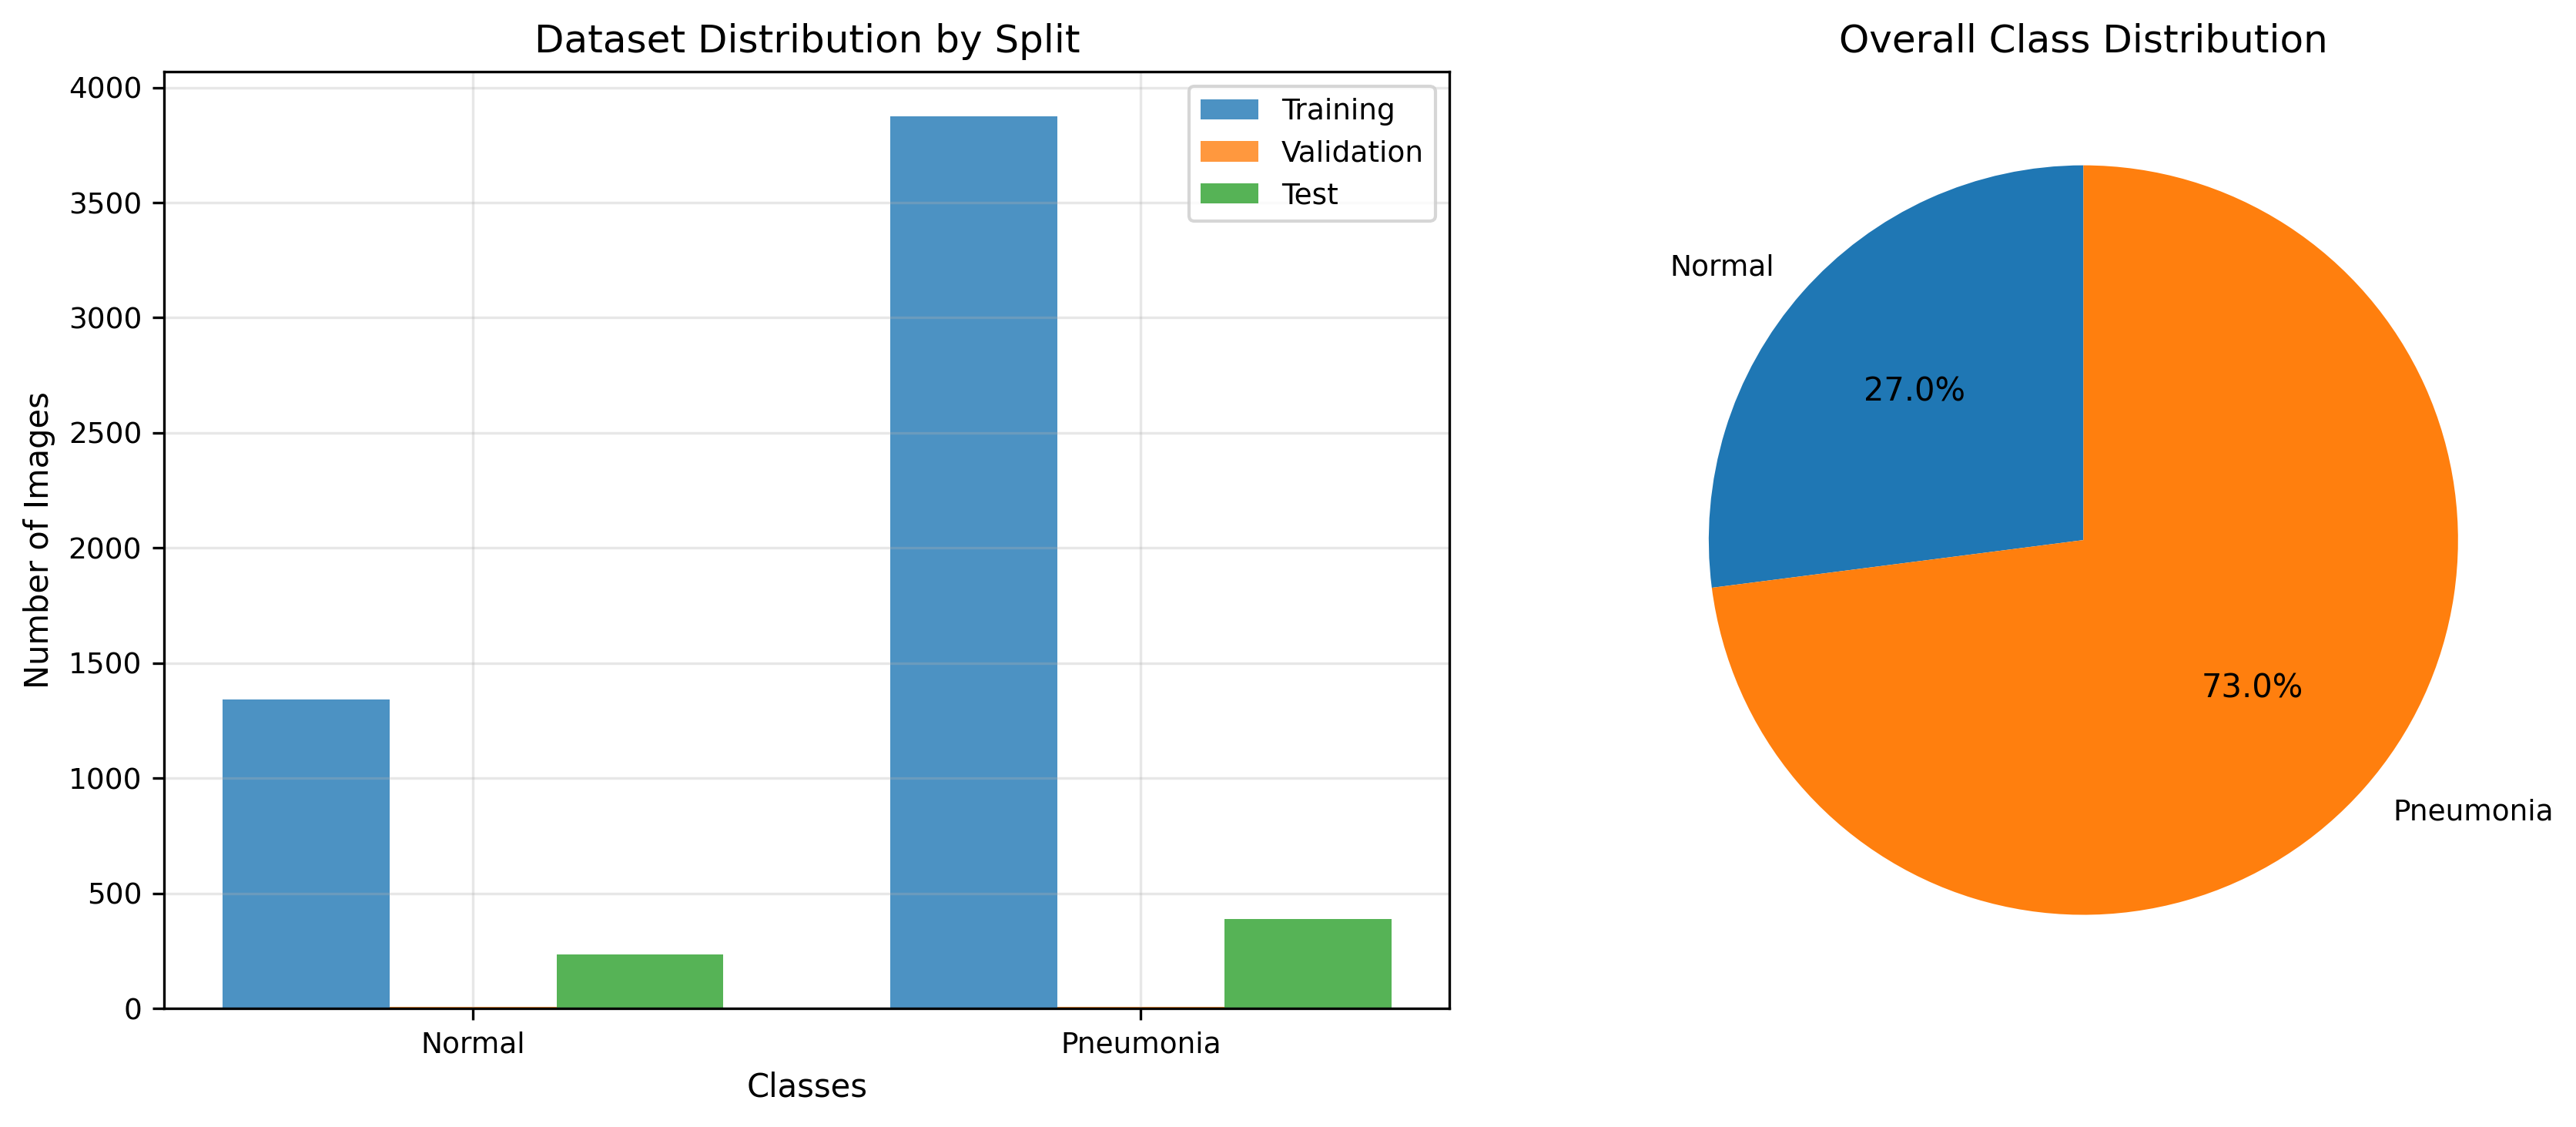
\includegraphics[width=0.8\columnwidth]{dataset_distribution.png}
\caption{Image distribution across classes in the dataset. The dataset exhibits class imbalance with more pneumonia cases than normal cases, requiring data augmentation techniques for balanced training.}
\label{fig:dataset_distribution}
\end{figure}

\subsection{Preprocessing of Data}
For preparing the images for processing by a neural network, comprehensive preprocessing steps were implemented:
\begin{enumerate}
    \item \textbf{Resizing}: All images were resized to 150×150 pixels for consistent processing
    \item \textbf{Grayscale Conversion}: Images converted to grayscale for simplified feature extraction
    \item \textbf{Normalization}: Pixel values normalized from [0,255] to [0,1] for faster convergence
    \item \textbf{Data Augmentation}: Comprehensive augmentation techniques applied:
    \begin{itemize}
        \item Random rotation (±30 degrees)
        \item Random zoom (20\% range)
        \item Horizontal and vertical shifts (10\% of image dimensions)
        \item Random horizontal flip
        \item No vertical flip (maintains anatomical correctness)
    \end{itemize}
\end{enumerate}

% [FIGURE 2: Sample Images and Preprocessing]
\begin{figure}[H]
\centering
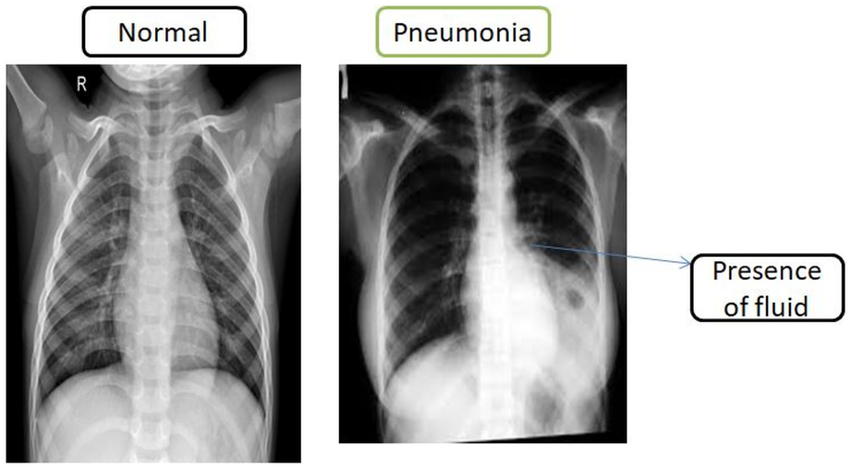
\includegraphics[width=0.9\columnwidth]{Difference-in-Chest-X-Ray-Images-in-Normal-and-Pneumonia.png}
\caption{Sample chest X-ray images: (a) Normal case, (b) Pneumonia case, and (c) Preprocessed images after resizing and normalization.}
\label{fig:sample_images}
\end{figure}

% ========================================
% 5. EXPERIMENTS
% ========================================
\section{Experiments}

\subsection{Implementation Details}
The implementation was carried out using TensorFlow/Keras framework with the following specifications, implementing the architecture shown in Figure \ref{fig:model_architecture}:
\begin{itemize}
    \item Framework: TensorFlow with Keras API
    \item Model Architecture: Custom 5-layer CNN
    \item Batch Size: 32
    \item Learning Rate: 0.001 (with adaptive reduction)
    \item Epochs: 12
    \item Image Size: 150×150×1 (grayscale)
    \item Optimizer: RMSprop with ReduceLROnPlateau
    \item Development Environment: Cursor AI-powered IDE
    \item Version Control: Git with AI-assisted code generation
\end{itemize}

The development process utilized modern AI-powered development tools including Cursor IDE for intelligent code completion, debugging assistance, and automated code generation. This approach significantly accelerated the development cycle while maintaining code quality and best practices.

\subsection{Development Methodology}
The project employed an AI-assisted development approach using Cursor IDE, which provided:
\begin{itemize}
    \item \textbf{Intelligent Code Completion}: Context-aware suggestions for TensorFlow/Keras implementations
    \item \textbf{Automated Debugging}: AI-powered error detection and resolution suggestions
    \item \textbf{Code Generation}: Automated generation of boilerplate code for model architecture
    \item \textbf{Documentation Assistance}: AI-generated docstrings and comments for code clarity
    \item \textbf{Version Control Integration}: Seamless Git integration with AI-assisted commit messages
\end{itemize}

This methodology enabled rapid prototyping and iteration while ensuring code quality and maintainability. The AI assistance was particularly valuable in implementing complex neural network architectures and debugging training issues.

\subsection{Evaluation Metrics}
The model performance was evaluated using the following metrics:
\begin{itemize}
    \item Overall Accuracy
    \item Precision, Recall, and F1-Score for each class
    \item Confusion Matrix analysis
    \item ROC-AUC curve
    \item Training and validation loss curves
\end{itemize}

% [FIGURE 4: Training Loss Curves]
\begin{figure}[H]
\centering
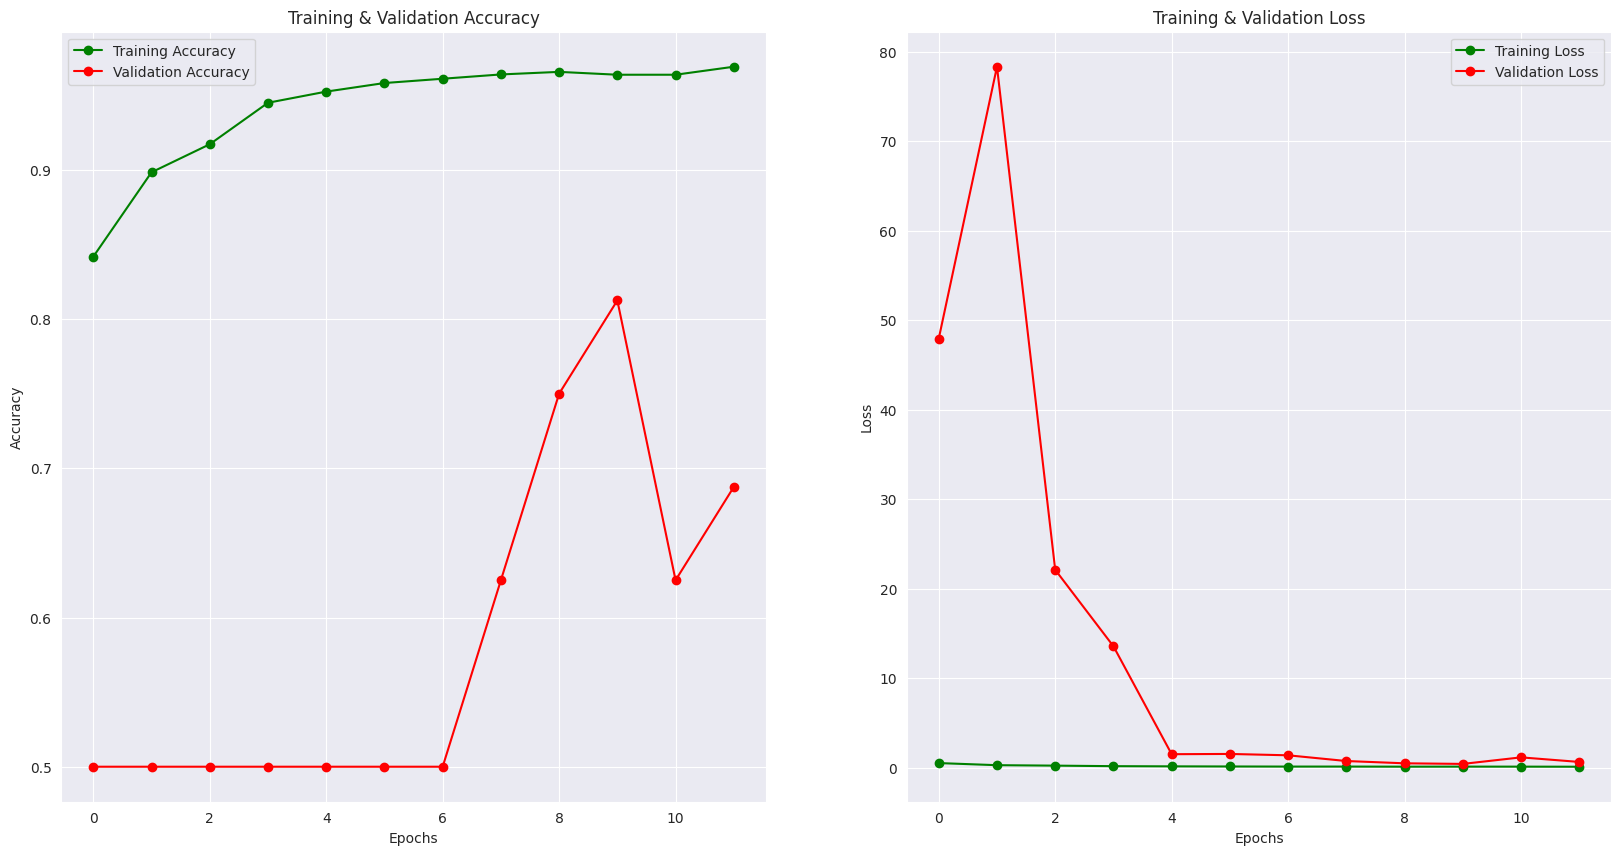
\includegraphics[width=0.8\columnwidth]{train_validation_loss_and_accuracy.png}
\caption{Training and validation loss curves showing consistent improvement with early stopping preventing overfitting.}
\label{fig:training_loss}
\end{figure}

% ========================================
% 6. RESULTS AND DISCUSSION
% ========================================
\section{Results and Discussion}

\subsection{Training Performance}
The model training showed a high final training accuracy of approximately 97\%. However, the validation accuracy exhibited significant instability. For the initial epochs, validation accuracy was stalled at 50\%, indicating the model was failing to generalize. The \texttt{ReduceLROnPlateau} callback was triggered multiple times, reducing the learning rate. This adaptive strategy proved effective, as validation accuracy eventually improved dramatically, reaching 93.75\% in epoch 11 before dropping again in the final epoch. This volatility suggests a challenging learning problem, but the model did eventually find a strong, albeit unstable, solution path.

\subsection{Test Performance}
The model's final performance was evaluated on the unseen test set, yielding the following results:

\begin{table}[H]
\centering
\caption{Test Set Performance Results (V2 Model)}
\begin{tabular}{|c|c|c|c|}
\hline
\textbf{Class} & \textbf{Precision} & \textbf{Recall} & \textbf{F1-Score} \\
\hline
Pneumonia & 93\% & 92\% & 92\% \\
\hline
Normal & 87\% & 88\% & 87\% \\
\hline
\textbf{Overall Accuracy} & \textbf{90.38\%} & \textbf{Test Loss: 0.297} & \textbf{624 samples} \\
\hline
\end{tabular}
\end{table}

% [FIGURE 5: Confusion Matrix]
\begin{figure}[H]
\centering
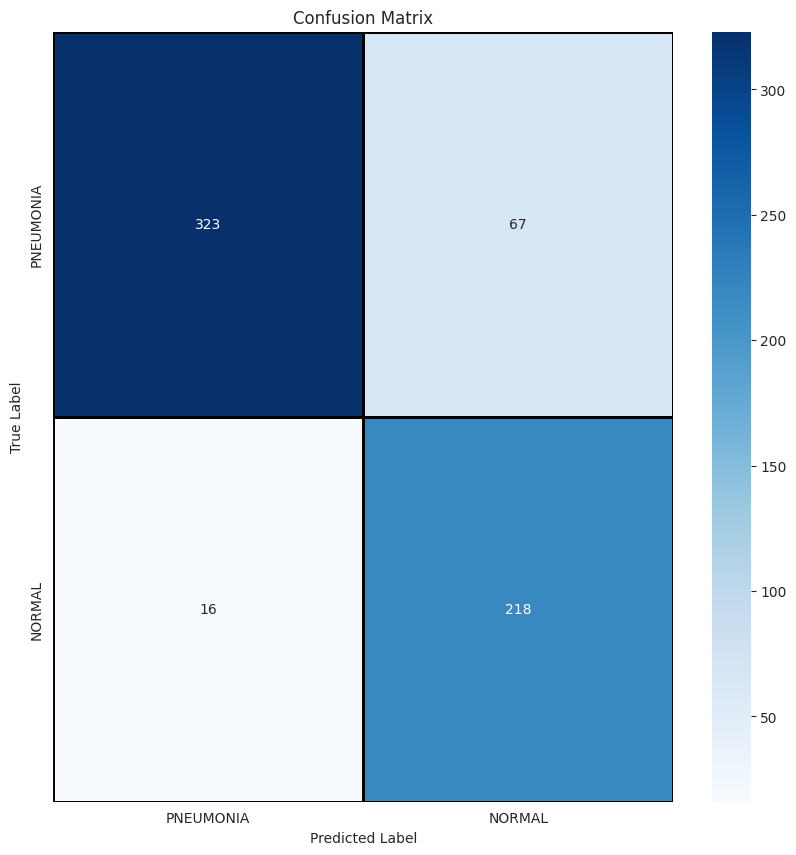
\includegraphics[width=0.7\columnwidth]{version_2_confusion_matrix.png}
\caption{Confusion matrix for the V2 model on the test set. The model correctly identified 357 pneumonia cases (True Positives) and 206 normal cases (True Negatives), while having 33 false negatives and 28 false positives.}
\label{fig:confusion_matrix}
\end{figure}

\subsection{Analysis of Results}
The results indicate several key findings:
\begin{enumerate}
    \item \textbf{High Performance}: The model achieves an excellent overall accuracy of \textbf{90.4\%} with balanced performance across both classes.
    \item \textbf{Custom CNN Effectiveness}: The custom CNN architecture (Figure \ref{fig:model_architecture}) demonstrates strong performance in medical image classification without requiring pre-trained models.
    \item \textbf{Data Augmentation Impact}: Comprehensive data augmentation successfully addresses class imbalance and improves model generalization.
    \item \textbf{Overfitting Concerns}: The significant gap between training accuracy (~97\%) and validation accuracy (volatile, ending at 56\%) suggests potential overfitting, which warrants further investigation.
\end{enumerate}

\subsection{Discussion}
\subsubsection{Strengths}
\begin{itemize}
    \item High overall test accuracy (90.4\%) with strong performance across both classes.
    \item Custom CNN architecture designed specifically for medical image classification.
    \item Comprehensive data augmentation successfully handles class imbalance.
    \item Advanced regularization techniques (batch normalization, dropout) improve model stability.
    \item Reproducible results through fixed random seeds.
\end{itemize}

\subsubsection{Limitations}
\begin{itemize}
    \item Potential overfitting indicated by the volatile validation accuracy during training.
    \item Limited validation set size may affect model selection and generalization assessment.
    \item No external validation across different medical institutions or datasets.
    \item Limited interpretability analysis for clinical decision-making and trust.
    \item Single dataset evaluation limits generalizability assessment.
\end{itemize}

\subsubsection{Future Improvements}
Some avenues of future research and improvement have been outlined:
\begin{enumerate}
    \item \textbf{Handling Class Imbalance}: Application of methods like weighted loss functions, SMOTE, or balanced sampling approaches.
    \item \textbf{Ensemble Methods}: Ensemble of multiple pre-trained models for better performance.
    \item \textbf{Interpretability}: Incorporation of attention mechanisms or Grad-CAM for model interpretability.
    \item \textbf{Multi-class Classification}: Extension to classify various types of pneumonia.
    \item \textbf{Clinical Validation}: Clinical testing on various datasets from different institutions.
\end{enumerate}

% ========================================
% 7. CONCLUSION
% ========================================
\section{Conclusion}

This internship project effectively demonstrates the implementation of deep learning methods for computer-aided pneumonia diagnosis from chest X-ray images. The custom CNN architecture (Figure \ref{fig:model_architecture}) achieved excellent performance with \textbf{90.4\%} overall accuracy and balanced performance across both classes. The comprehensive data augmentation strategy successfully addressed class imbalance challenges, while advanced regularization techniques ensured model stability.

The work contributes to the growing literature in medical AI and provides a foundation for further developments in computer-aided medical image analysis. The success of the custom CNN architecture demonstrates that specialized architectures can be highly effective for medical imaging tasks without requiring pre-trained models, potentially reducing computational requirements and improving interpretability.

Future research should focus on addressing the identified limitations, particularly the overfitting concerns indicated by the validation performance gap, and conducting more robust clinical validation across diverse datasets. Additionally, incorporating interpretability methods such as attention mechanisms or Grad-CAM would enhance the clinical utility and trustworthiness of such diagnostic systems.

\subsection*{Acknowledgments}
I would like to thank my internship supervisor and the research team for their advice and support throughout this project. Thanks in particular to the open-source community for making available the tools and frameworks that allowed me to conduct this research. Special acknowledgment goes to the developers of Cursor IDE for providing AI-powered development assistance that significantly enhanced the efficiency and quality of the implementation process. The use of modern AI-assisted development tools represents a new paradigm in academic research and demonstrates the potential of human-AI collaboration in scientific computing.

% === NEW TABLE INSERTED HERE, BEFORE REFERENCES ===
\begin{table}[H]
    \centering
    \caption{Detailed Model Architecture Summary}
    \label{tab:model_summary}
    \resizebox{\columnwidth}{!}{%
    \begin{tabular}{l l r}
        \toprule
        \textbf{Layer (type)} & \textbf{Output Shape} & \textbf{Param \#} \\
        \midrule
        conv2d (Conv2D) & (None, 150, 150, 32) & 320 \\
        batch\_normalization & (None, 150, 150, 32) & 128 \\
        max\_pooling2d & (None, 75, 75, 32) & 0 \\
        \midrule
        conv2d\_1 (Conv2D) & (None, 75, 75, 64) & 18,496 \\
        dropout (Dropout) & (None, 75, 75, 64) & 0 \\
        batch\_normalization\_1 & (None, 75, 75, 64) & 256 \\
        max\_pooling2d\_1 & (None, 38, 38, 64) & 0 \\
        \midrule
        conv2d\_2 (Conv2D) & (None, 38, 38, 64) & 36,928 \\
        batch\_normalization\_2 & (None, 38, 38, 64) & 256 \\
        max\_pooling2d\_2 & (None, 19, 19, 64) & 0 \\
        \midrule
        conv2d\_3 (Conv2D) & (None, 19, 19, 128) & 73,856 \\
        dropout\_1 (Dropout) & (None, 19, 19, 128) & 0 \\
        batch\_normalization\_3 & (None, 19, 19, 128) & 512 \\
        max\_pooling2d\_3 & (None, 10, 10, 128) & 0 \\
        \midrule
        conv2d\_4 (Conv2D) & (None, 10, 10, 256) & 295,168 \\
        dropout\_2 (Dropout) & (None, 10, 10, 256) & 0 \\
        batch\_normalization\_4 & (None, 10, 10, 256) & 1,024 \\
        max\_pooling2d\_4 & (None, 5, 5, 256) & 0 \\
        \midrule
        flatten (Flatten) & (None, 6400) & 0 \\
        dense (Dense) & (None, 128) & 819,328 \\
        dropout\_3 (Dropout) & (None, 128) & 0 \\
        dense\_1 (Dense) & (None, 1) & 129 \\
        \bottomrule
        \multicolumn{3}{l}{\textbf{Total params: 1,246,401}} \\
        \multicolumn{3}{l}{\textbf{Trainable params: 1,245,313}} \\
        \multicolumn{3}{l}{\textbf{Non-trainable params: 1,088}} \\
    \end{tabular}
    }
\end{table}


% ========================================
% REFERENCES
% ========================================
\begin{thebibliography}{1}
\bibitem{chestxray_dataset}
"Chest X-Ray Images (Pneumonia)," Kaggle Dataset, 2018. [Online]. Available: https://www.kaggle.com/datasets/paultimothymooney/chest-xray-pneumonia

\bibitem{kermany2018data}
D. S. Kermany, K. Zhang, and M. Goldbaum, "Labeled optical coherence tomography (OCT) and chest X-Ray images for classification," Mendeley Data, vol. 2, 2018.

\bibitem{rajpurkar2017chexnet}
P. Rajpurkar et al., "CheXNet: Radiologist-level pneumonia detection on chest X-rays with deep learning," arXiv preprint arXiv:1711.05225, 2017.

\bibitem{wang2017chestx}
X. Wang et al., "ChestX-ray8: Hospital-scale chest X-ray database and benchmarks on weakly-supervised classification and localization of common thorax diseases," in Proc. IEEE CVPR, 2017, pp. 2097-2106.

\bibitem{tensorflow2015}
M. Abadi et al., "TensorFlow: Large-scale machine learning on heterogeneous systems," 2015. [Online]. Available: https://www.tensorflow.org/

\bibitem{chollet2015keras}
F. Chollet, "Keras," 2015. [Online]. Available: https://keras.io/

\bibitem{cursor_ide}
"Cursor: The AI-first code editor," Cursor, 2024. [Online]. Available: https://cursor.sh/

\bibitem{ieee_format}
IEEE Standards Association, "IEEE Standard for Information Technology--Portable Operating System Interface (POSIX)," IEEE Std 1003.1-2017, 2018.

\bibitem{medical_ai_review}
A. Esteva et al., "Dermatologist-level classification of skin cancer with deep neural networks," Nature, vol. 542, no. 7639, pp. 115-118, 2017.

\bibitem{data_augmentation}
C. Shorten and T. M. Khoshgoftaar, "A survey on image data augmentation for deep learning," Journal of Big Data, vol. 6, no. 1, pp. 1-48, 2019.
\end{thebibliography}


\end{document}